\documentclass[
	% -- opções da classe memoir --
	12pt,				% tamanho da fonte
	openright,			% capítulos começam em pág ímpar (insere página vazia caso preciso)
	oneside,			% para impressão em recto e verso. Oposto a oneside
	a4paper,			% tamanho do papel. 
	% -- opções da classe abntex2 --
	%chapter=TITLE,		% títulos de capítulos convertidos em letras maiúsculas
	%section=TITLE,		% títulos de seções convertidos em letras maiúsculas
	%subsection=TITLE,	% títulos de subseções convertidos em letras maiúsculas
	%subsubsection=TITLE,% títulos de subsubseções convertidos em letras maiúsculas
	% -- opções do pacote babel --
	english,			% idioma adicional para hifenização
	brazil,				% o último idioma é o principal do documento
	]{abntex2}


% ---
% PACOTES
% ---

% Pacotes fundamentais 
\usepackage{lmodern}			% Usa a fonte Latin Modern
\usepackage[T1]{fontenc}		% Selecao de codigos de fonte.
\usepackage[utf8]{inputenc}		% Codificacao do documento (conversão automática dos acentos)
\usepackage{indentfirst}		% Indenta o primeiro parágrafo de cada seção.
\usepackage{color}				% Controle das cores
\usepackage{graphicx}			% Inclusão de gráficos
\usepackage{microtype} 			% para melhorias de justificação
\usepackage{UFAC} 				% fomato específico TCC da UFAC [Desenvolvido por P. Otávio]
\usepackage{float}

% Pacotes adicionais, usados no anexo do modelo de folha de identificação
\usepackage{multicol}
\usepackage{multirow}
	
% Pacotes adicionais, usados apenas no âmbito do Modelo Canônico do abnteX2
\usepackage{lipsum}				% para geração de dummy text

% Pacotes de citações
\usepackage[brazilian,hyperpageref]{backref}	 % Paginas com as citações na bibl
\usepackage[alf]{abntex2cite}	% Citações padrão ABNT


% --- 
% CONFIGURAÇÕES DE PACOTES
% --- 

% Configurações do pacote backref
% Usado sem a opção hyperpageref de backref
\renewcommand{\backrefpagesname}{Citado na(s) página(s):~}
% Texto padrão antes do número das páginas
\renewcommand{\backref}{}
% Define os textos da citação
\renewcommand*{\backrefalt}[4]{
	\ifcase #1 %
		Nenhuma citação no texto.%
	\or
		Citado na página #2.%
	\else
		Citado #1 vezes nas páginas #2.%
	\fi}%

% Informações de dados para CAPA e FOLHA DE ROSTO
\titulo{Relatório de Projeto Final da Disciplina de Automação de Sistemas}
% ---------------------------------------------------
\autor{	Nathalia Nascimento \\
		Luiz Felipe Fontes}
% ---------------------------------------------------
\local{Rio de Janeiro}
\data{2021}
\tipotrabalho{Relatório técnico}
% O preambulo deve conter o tipo do trabalho, o objetivo, 
% o nome da instituição e a área de concentração 
\preambulo{Relatório de Projeto Final apresentado à Disciplina de Automação de Sistemas do Curso de Engenharia de Controle e Automação do CEFET-RJ, como requisito parcial para aprovação.}

% Configurações de aparência do PDF final

% alterando o aspecto da cor azul
\definecolor{blue}{RGB}{41,5,195}

% informações do PDF
\makeatletter
\hypersetup{
     	%pagebackref=true,
		pdftitle={\@title}, 
		pdfauthor={\@author},
    	pdfsubject={\imprimirpreambulo},
	    pdfcreator={LaTeX with abnTeX2},
		pdfkeywords={abnt}{latex}{abntex}{abntex2}{relatório técnico}, 
		colorlinks=true,       		% false: boxed links; true: colored links
    	linkcolor=black,          	% color of internal links
    	citecolor=black,        		% color of links to bibliography
    	filecolor=black,      		% color of file links
		urlcolor=blue,
		bookmarksdepth=4
}
\makeatother

% Espaçamentos entre linhas e parágrafos 

% O tamanho do parágrafo é dado por:
\setlength{\parindent}{1.3cm}

% Controle do espaçamento entre um parágrafo e outro:
\setlength{\parskip}{0.2cm}  % tente também \onelineskip

% compila o indice
\makeindex

% Início do documento
\begin{document}

% Seleciona o idioma do documento (conforme pacotes do babel)
%\selectlanguage{english}
\selectlanguage{brazil}

% Retira espaço extra obsoleto entre as frases.
\frenchspacing 

% ----------------------------------------------------------
% ELEMENTOS PRÉ-TEXTUAIS
% ----------------------------------------------------------

% Capa
\imprimircapa

% Folha de rosto
% (o * indica que haverá a ficha bibliográfica)
\imprimirfolhaderosto*

% inserir o sumario
\pdfbookmark[0]{\contentsname}{toc}
\tableofcontents*
\cleardoublepage


% ----------------------------------------------------------
% ELEMENTOS TEXTUAIS
% ----------------------------------------------------------
\textual


\chapter{Introdução}
%\lipsum[4]
A disciplina de Automação de Sistemas têm como propósito introduzir os alunos dos cursos de engenharia do CEFET-RJ acerca de conceitos da área da automação de sistemas industriais como os controladores lógico Programáveis (CLPs), atuadores, sistemas supervisórios e redes industriais.  

Esse relatório apresenta o projeto elaborado como avaliação parcial para aprovação na disciplina de Automação de Sistemas. No projeto  é desenvolvimdo um sistema de manipulação de caixas numa linha de produção. O problema é caracterizado por duas esteiras rolantes e um braço mecânico para sustentação e movimentação das caixas entre as esteiras. Ademais, o sistema é composto por elementos de entradas para a manipulação do operador e atuadores.  

\chapter{Tarefa Proposta}

A tarefa proposta para resolução ilustra uma linha de produção caracterizada por caixas transportadas em esteiras rolantes, um braço mecânico e um painel de controle. Na imagem abaixo está uma representação.

\begin{figure}[htb!]
\centering
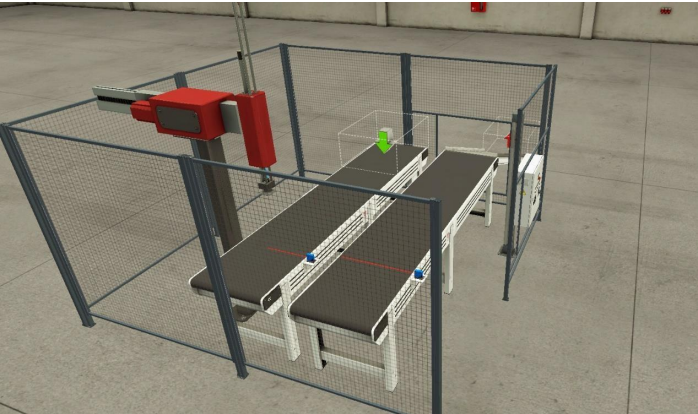
\includegraphics[width=0.5\linewidth]{Imagens/i1.PNG}
\caption{Projeto proposto}
\label{fig:problema}
\end{figure}

As esteiras são acionadas em direções opostas e o sistema precisa atender aos requisitos seguintes:

\begin{itemize}
    \item A esteira de entrada é acionada quando o sistema é ligado e deve
    parar quando a peça chegar no sensor abaixo do robô.
    \item A esteira de saída deve ser acionada quando houver peças nela.
    \item Enquanto houver peça presas ao robô, as esteiras devem permanecer
    paradas.
    \item O movimento do robô é para frente e para trás (move x) e para cima e
    para baixo (move Z).
    \item O robô deve voltar para sua posição de origem para pegar a próxima peça
\end{itemize}

As ferramentas de desenvolvimento e simulação sugeridas são o TIA Portal ou Master Tool IEC \cite{mastertool2009}, Factory I/O \cite{factoryio} e PLC Sim \cite{plcsim}. Além disso, o software precisa ser desenvolvido em linguagem Ladder e as entradas da planta são caracterizadas pelos itens abaixo:

\begin{itemize}
    \item Botão de início do sistema (Start);
    \item Botão de parada do sistema (Stop);
    \item Botão de reset da contagem;
    \item Botão de emergência;
    \item Sensor 1: Na esteira de entrada;
    \item Sensor 2: Na esteira de saída;
    \item Sensor 3: Na garra do robô;
\end{itemize}

O painel de controle deve apresentar as funcionalidades de acionar e parar o sistema, resetar a contagem, acionar a emergência e mostrar o número de peças contabilizadas. Além disso, o painel deve conter lâmpadas que precisam acender nas seguintes ocasiões:
\begin{itemize}
\item \textbf{Lâmpada de parada (Stop light)}: Acesa quando o sistema não estiver em operação ou o botão \textit{Stop} for acionado.
\item \textbf{Lâmpada de início (Start light)}: Acesa quando o botão \textit{Start} é acionado e o sistema está em operação.
\item \textbf{Lâmpada de emergência}: Acesa quando o botão de emergência é acionado.
\end{itemize}

Ademais, quando a contagem de caixas atingir o número vinte, um alarme é disparado para alertar o operador sobre o limite de caixas e o conteúdo do display se mantém fixo até que a contagem seja reiniciada.

\chapter{Relato do Projeto}

Foram tomadas duas iniciativas para resolução da tarefa. A primeira, e principal delas, foi desenvolvida com os recursos dos softwares TIA Portal, PLC Sim e Factory I/O. 

Os simuladores facilitaram o teste do software e a visualização da linha de produção em operação .Os arquivos do projeto desenvolvido no TIA Portal e o script principal estão disponível na seção [\ref{anexos}].

A seguir são expostas imagens da simulação na ferramenta Factory I/O e a interface homem máquina (IHM) elaborada para o controle manual do operador. 

\begin{figure}[H]
\centering
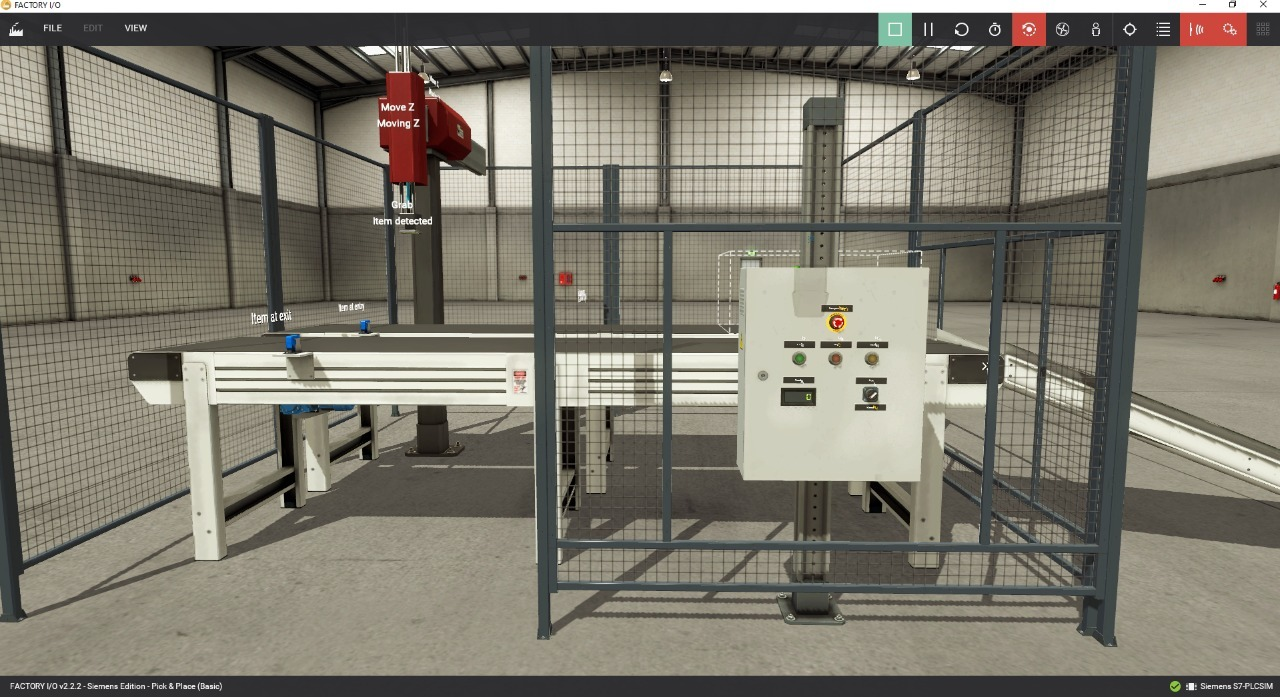
\includegraphics[width=1\linewidth]{Imagens/i2.jpeg}
\caption{Imagem da simulação no Factory I/O}
\label{fig:simulaçao_1}
\end{figure}

\begin{figure}[H]
\centering
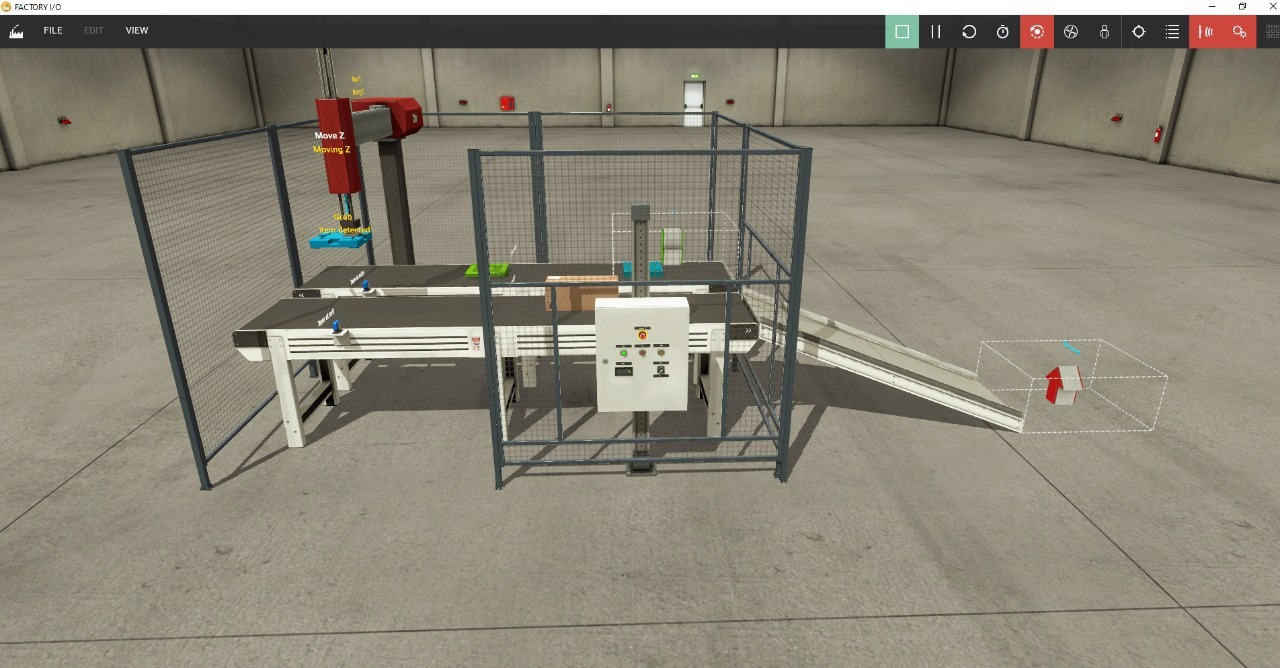
\includegraphics[width=1\linewidth]{Imagens/i3.jpeg}
\caption{Imagem da simulação no Factory I/O}
\label{fig:simulaçao_2}
\end{figure}

\begin{figure}[H]
\centering
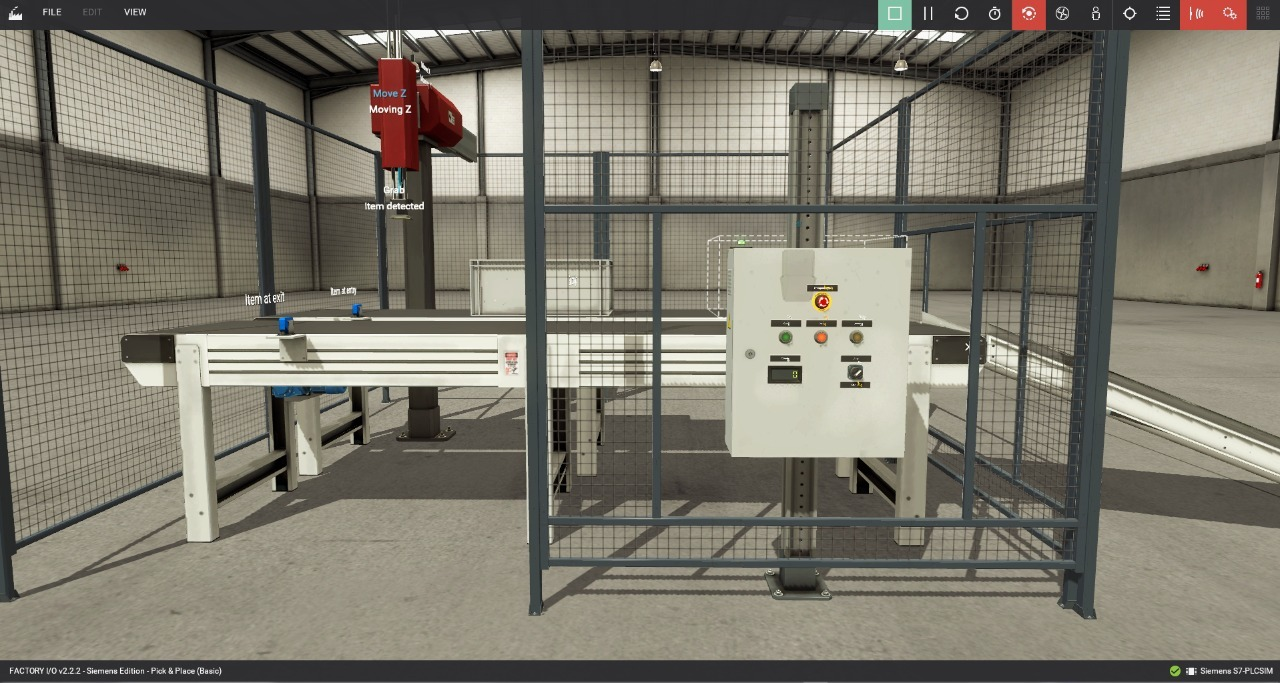
\includegraphics[width=1\linewidth]{Imagens/i4.jpeg}
\caption{Imagem da simulação no Factory I/O}
\label{fig:simulaçao_3}
\end{figure}

\begin{figure}[H]
\centering
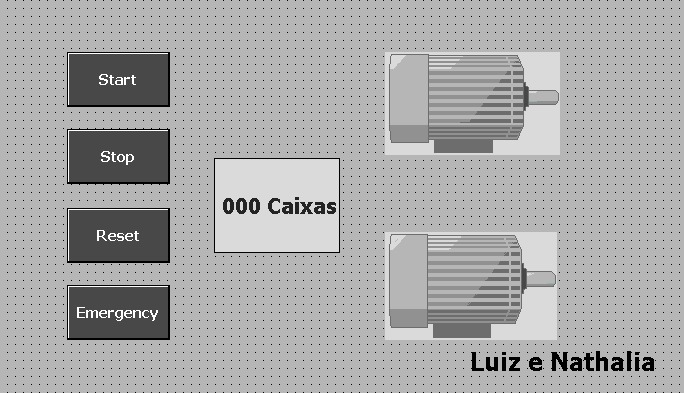
\includegraphics[width=0.5\linewidth]{Imagens/i6.jpeg}
\caption{IHM desenvolvido no TIA Portal}
\label{fig:ihm_1}
\end{figure}

Uma abordagem alternativa foi baseada na ferramenta Master Tool IEC e não contou com o recurso de simulação do Factory I/O. Nesse caso, o teste foi ministrado de maneira simplificada utilizando as funcionalidades de simulação de código no Master Tool IEC e a interface homem máquina (IHM) desenvolvida no mesmo.
A estratégia aqui foi a de destrinchar os passos envolvidos na locomoção da garra e representá-los graficamente na IHM.  

O sensor 3 foi suprimido na interface gráfica e substituído por um indicador de objeto na garra. O alarme sonoro também foi substituído por um indicador visual. Como a natureza do problema da locomoção do braço mecânico foi tratada digitalmente, ou seja, desconsiderando utilização de portas analógicas, foram inseridos indicadores de movimento do braço na IHM. Ademais, a fim de forçar a resposta dos sensores foram adicionados botões para comutar o estado dessas entradas, como um artifício de teste.

O script detalhado e o projeto estabelecido no Master Tool IEC estão disponíveis na seção [\ref{anexos}]. Adiante as imagens demonstra a IHM e os testes da operação.

\begin{figure}[H]
\centering
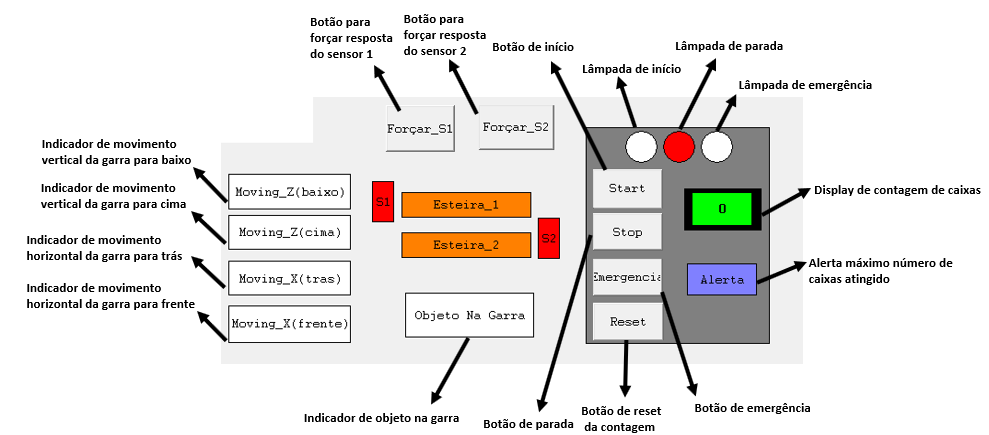
\includegraphics[width=1\linewidth]{Imagens/i7.PNG}
\caption{IHM desenvolvido no Master Tool IEC}
\label{fig:ihm_2}
\end{figure}

\begin{figure}[H]
\centering
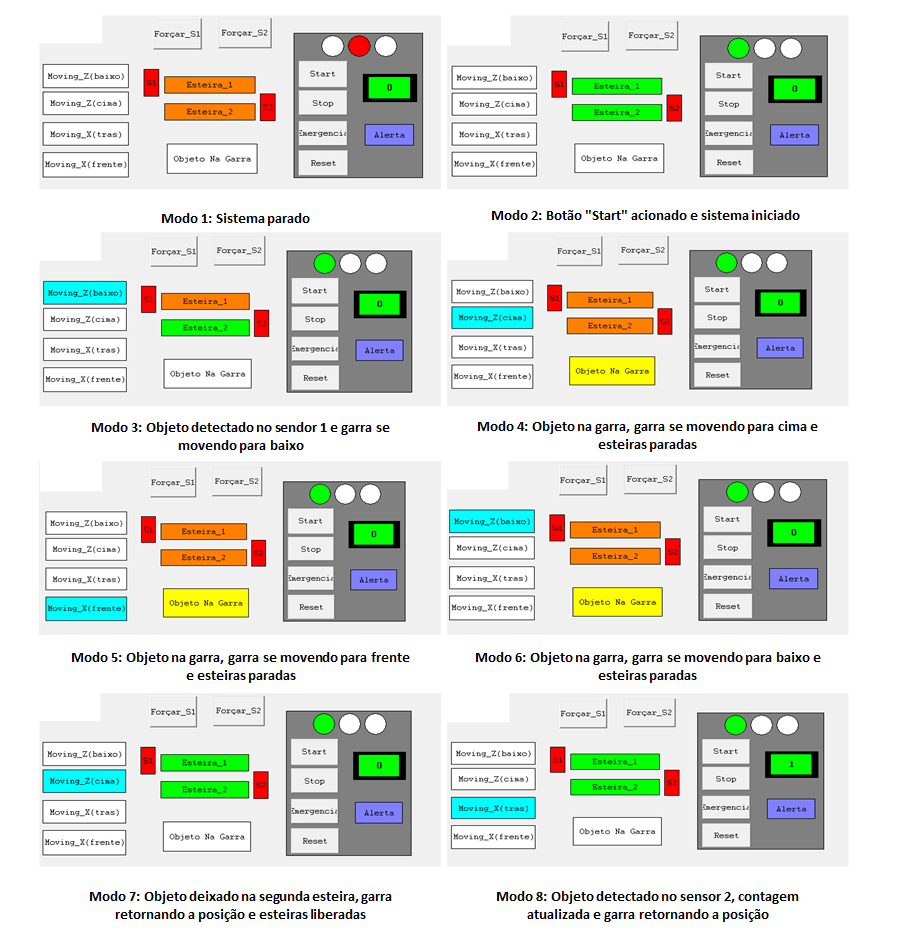
\includegraphics[width=1\linewidth]{Imagens/i8.png}
\caption{Sistema em operação}
\label{fig:sis}
\end{figure}

Em ambas abordagens as descrições abaixo em relação aos elementos da IHM são válidas:
\begin{itemize}
    \item \textbf{Botão Start}: Inicia o sistema e aciona a luz de sistema operante;
    \item \textbf{Botão Stop}: Paralisa a planta e aciona a luz de parada;
    \item \textbf{Botão Reset}: Reinicia a contagem de caixas;
    \item \textbf{Botão Emergência}: Aciona a luz de emergência e trava o sistema;
    \item \textbf{Display}: Demonstra a contagem das caixas;
\end{itemize}

As intruções para operação são especificadas a seguir:
\begin{enumerate}
    \item Para ligar o sistema, acione o botão "Start"
    \item Para desligar o sistema, acione o botão "Stop"
    \item Para travar o sistema, acione o botão "Emergência"/"Emergency"
    \item Para resetar a contagem de caixas no display, acione o botão "Reset"
\end{enumerate}

\chapter{Sugestão de Hardware}

Esse tópico visa apresentar algumas sugestões de hardware para a implementação do projeto descrito num ambiente físico. 

\section{Controlador Lógico Programável (CLP)}

O controlador sugerido é o S7 1200 \cite{s71200manual2012}. Algumas das características de sua CPU, além de um microprocessador, são uma fonte integrada, circuitos de entrada/saída e entradas analógicas.

A CPU é adaptada para comunicação em rede PROFINET e módulos adicionais podem ser adquiridos para comunicação PROFIBUS, GPRS, RS485, RS232, IEC, DNP3 e redes WDC.

\begin{figure}[H]
\centering
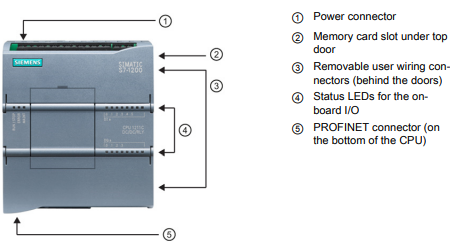
\includegraphics[width=1\linewidth]{Imagens/i9.PNG}
\caption{Controlador lógico programável S7 1200}
\label{fig:clp_sugerido}
\end{figure}

\section{Interface Homem Máquina (IHM)}

Tendo em vista a simplicidade do sistema descrito em relação a arranjos industriais mais complexos, é sugerida uma interface homem máquina básica dentre aquelas disponíveis para utilização com o CLP S7 1200. A KTP700 Basic é a opção viável nesse caso, possuindo tela \textit{touch screen} de 7'' e 8 chaves configuráveis. O dispositivo tem uma resolução de 800x480 e opera com até 800 TAGS.

\begin{figure}[H]
\centering
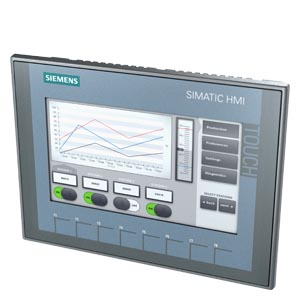
\includegraphics[width=0.5\linewidth]{Imagens/i10.jpg}
\caption{Interface homem máquina KTP700 Basic}
\label{fig:ihm_sugerida}
\end{figure}

\chapter{Conclusões}

O conteúdo exposto no relatório visa apresentar uma solução para a tarefa de criação de uma linha de produção completamente automatizada, guiando o leitor em termos dos recursos utilizados para desenvolvimento do sistema e a viabilidade de construção do mesmo. 

As ferramentas computacionais apresentadas durante as aulas da disciplina de Automação de Sistemas foram utilizadas para estruturar o sistema e testá-lo em um ambiente virtual. Ademais as sugestões de hardware possibilitam a implementação futura do projeto num contexto físico.

Os conteúdos ministrados na disciplina de Automação de Sistemas foram cruciais para o desenvolvimento e facilitaram a busca por soluções efetivas. 


\chapter{Anexos} \label{anexos}
\begin{itemize}
    \item Script principal desenvolvido no TIA Portal
    \\
    \\
    \item Script principal desenvolvido no Master Tool IEC
    \\
    \\
    \item Projeto completo desenvolvido no TIA Portal
    \\
    \\
    \item Projeto completo desenvolvido no Master Tool IEC
\end{itemize}

% ----------------------------------------------------------
% ELEMENTOS PÓS-TEXTUAIS
% ----------------------------------------------------------
\postextual

% ----------------------------------------------------------
% Referências bibliográficas
% ----------------------------------------------------------

\bibliography{referencias}

\end{document}
